\section{Simulation Study: Selected results}
\begin{figure}[h]
\caption{Emission distribution: Precision}
    \centering
    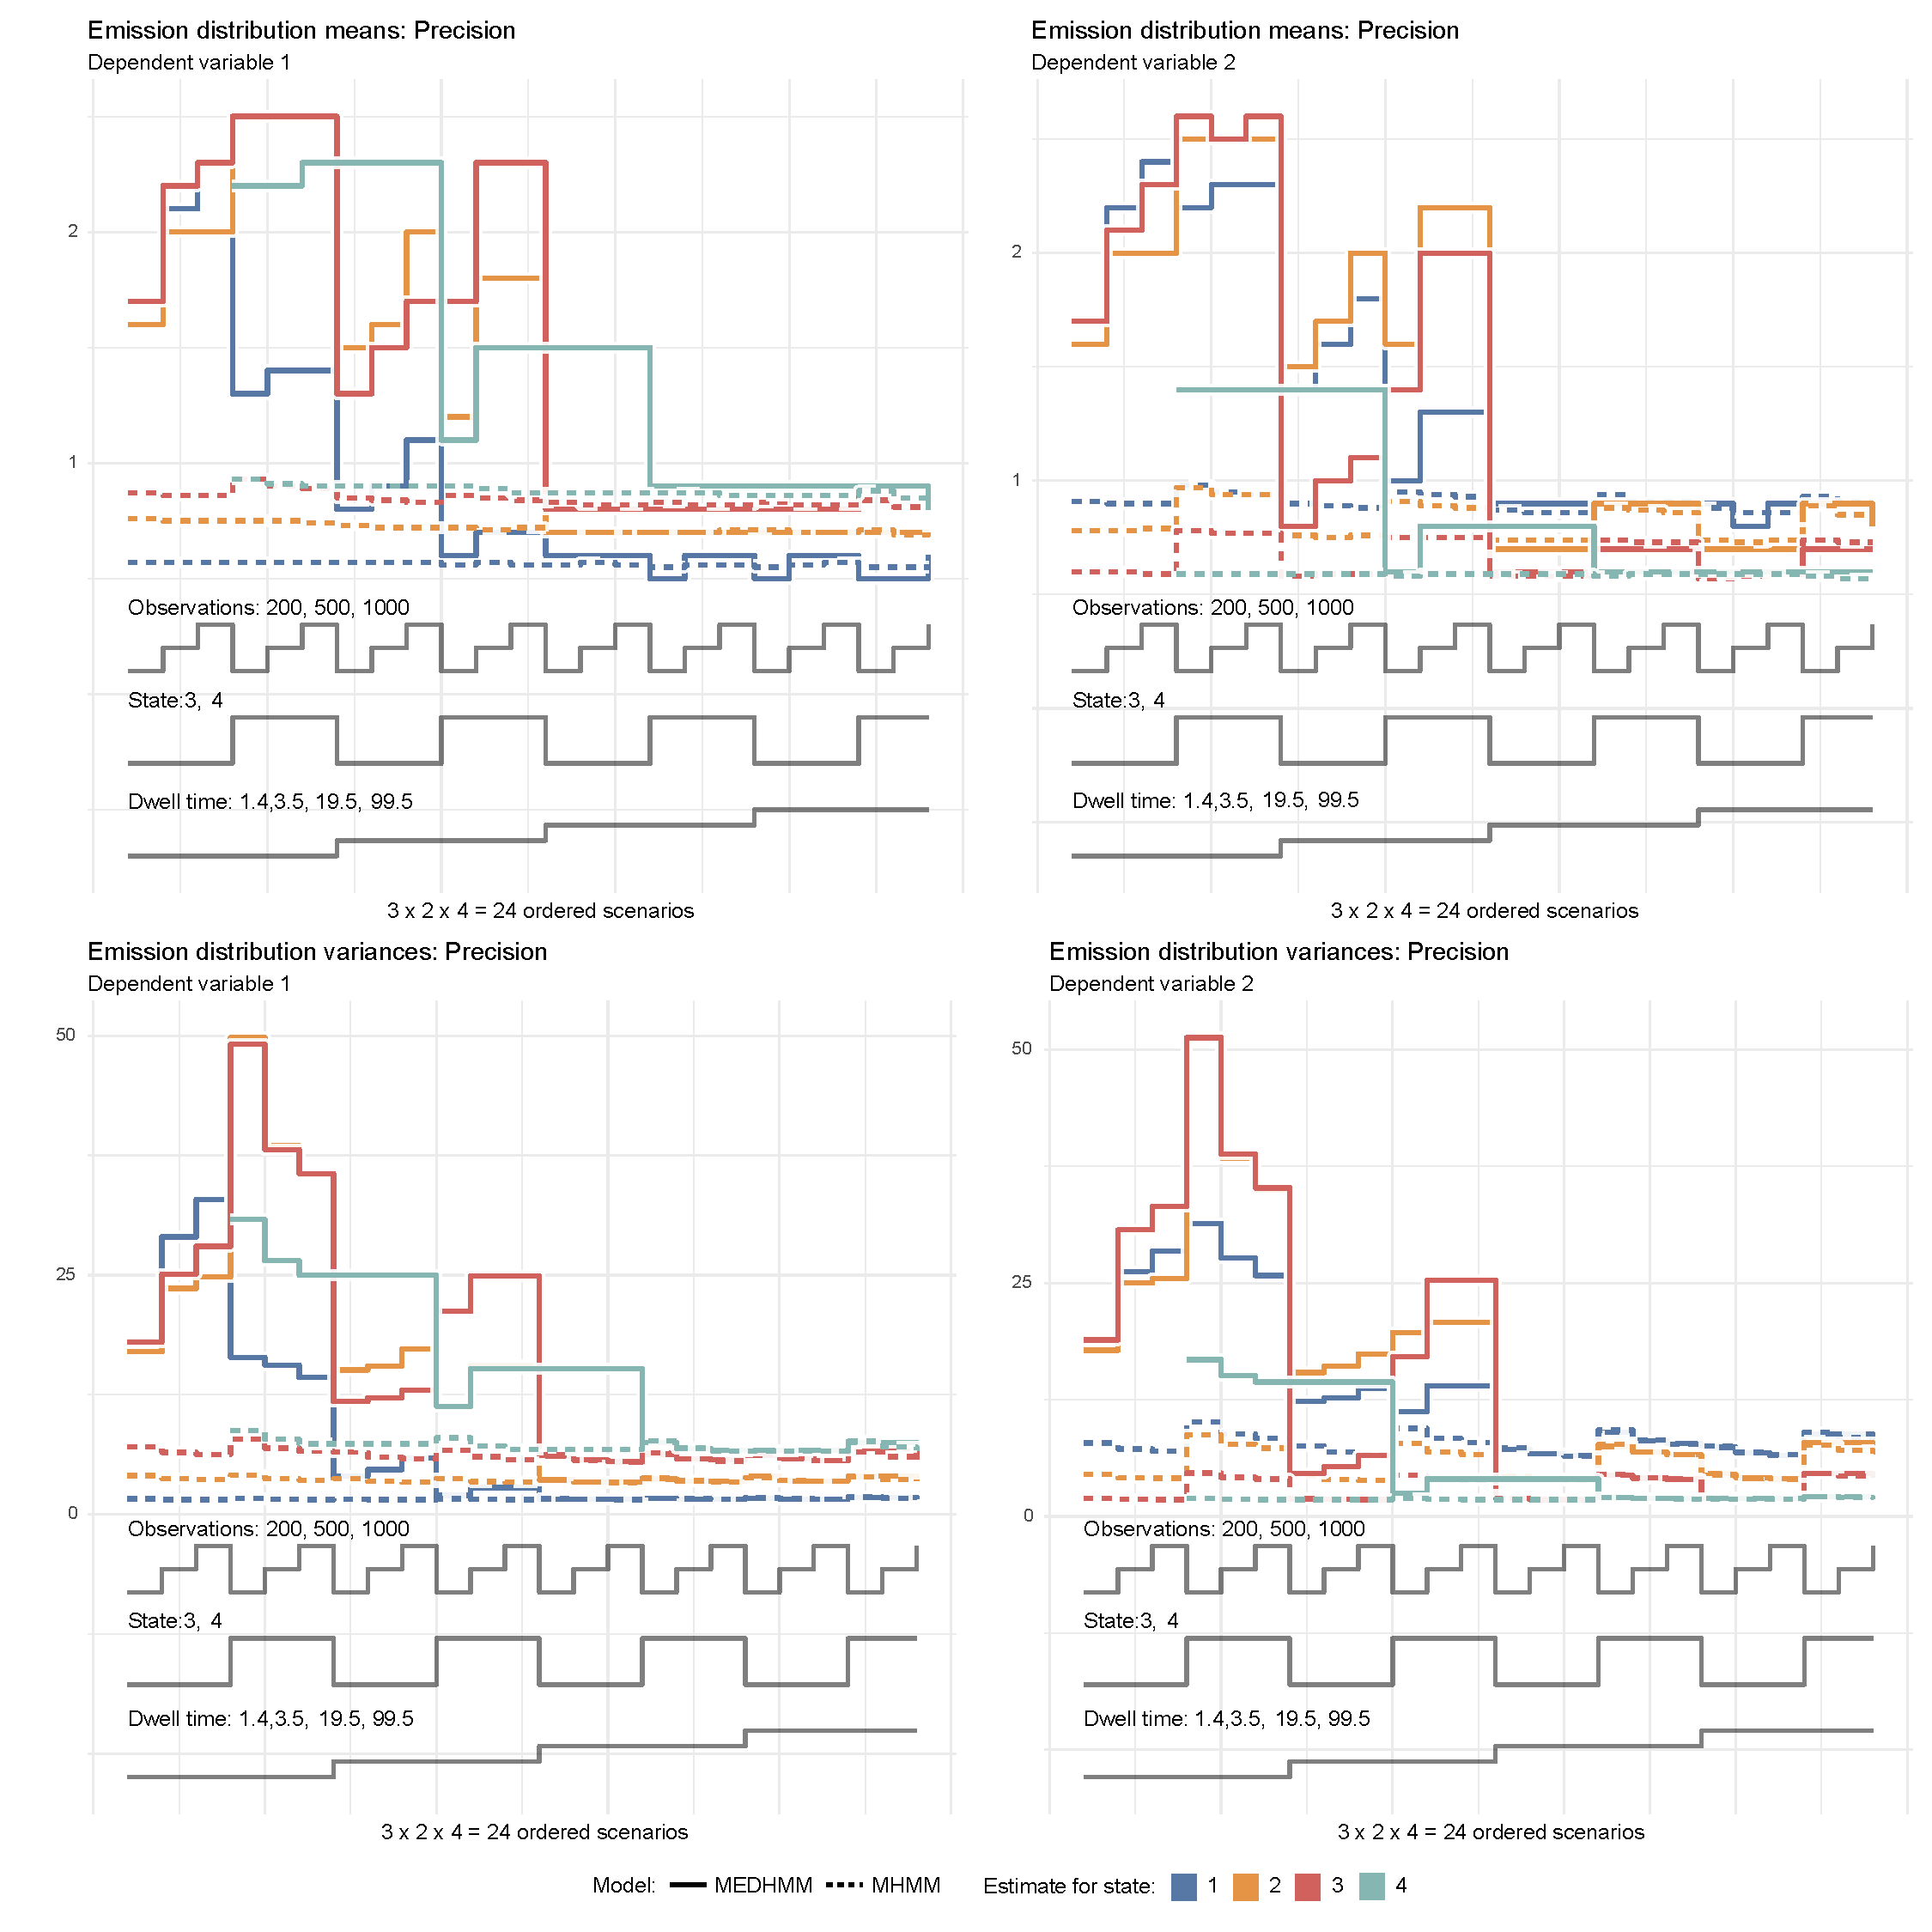
\includegraphics[width=0.75\textwidth]{graphics/emiss_sd.pdf}
    \label{prec_emiss}
    \flushleft
    \footnotesize
    \justifying
     Plots illustrate the empirical standard errors (precision) of each emission distribution means (first row) and emission variances (second row) for every simulation scenario (note that the additional scenario with varying dwell time is omitted). Each colour represent the state-specific emission mean parameters and line
type is the model indicator.
\end{figure}

%to appendix
\begin{figure}[h]
\caption{Emission distribution means: Coverage(\%)}
    \centering
    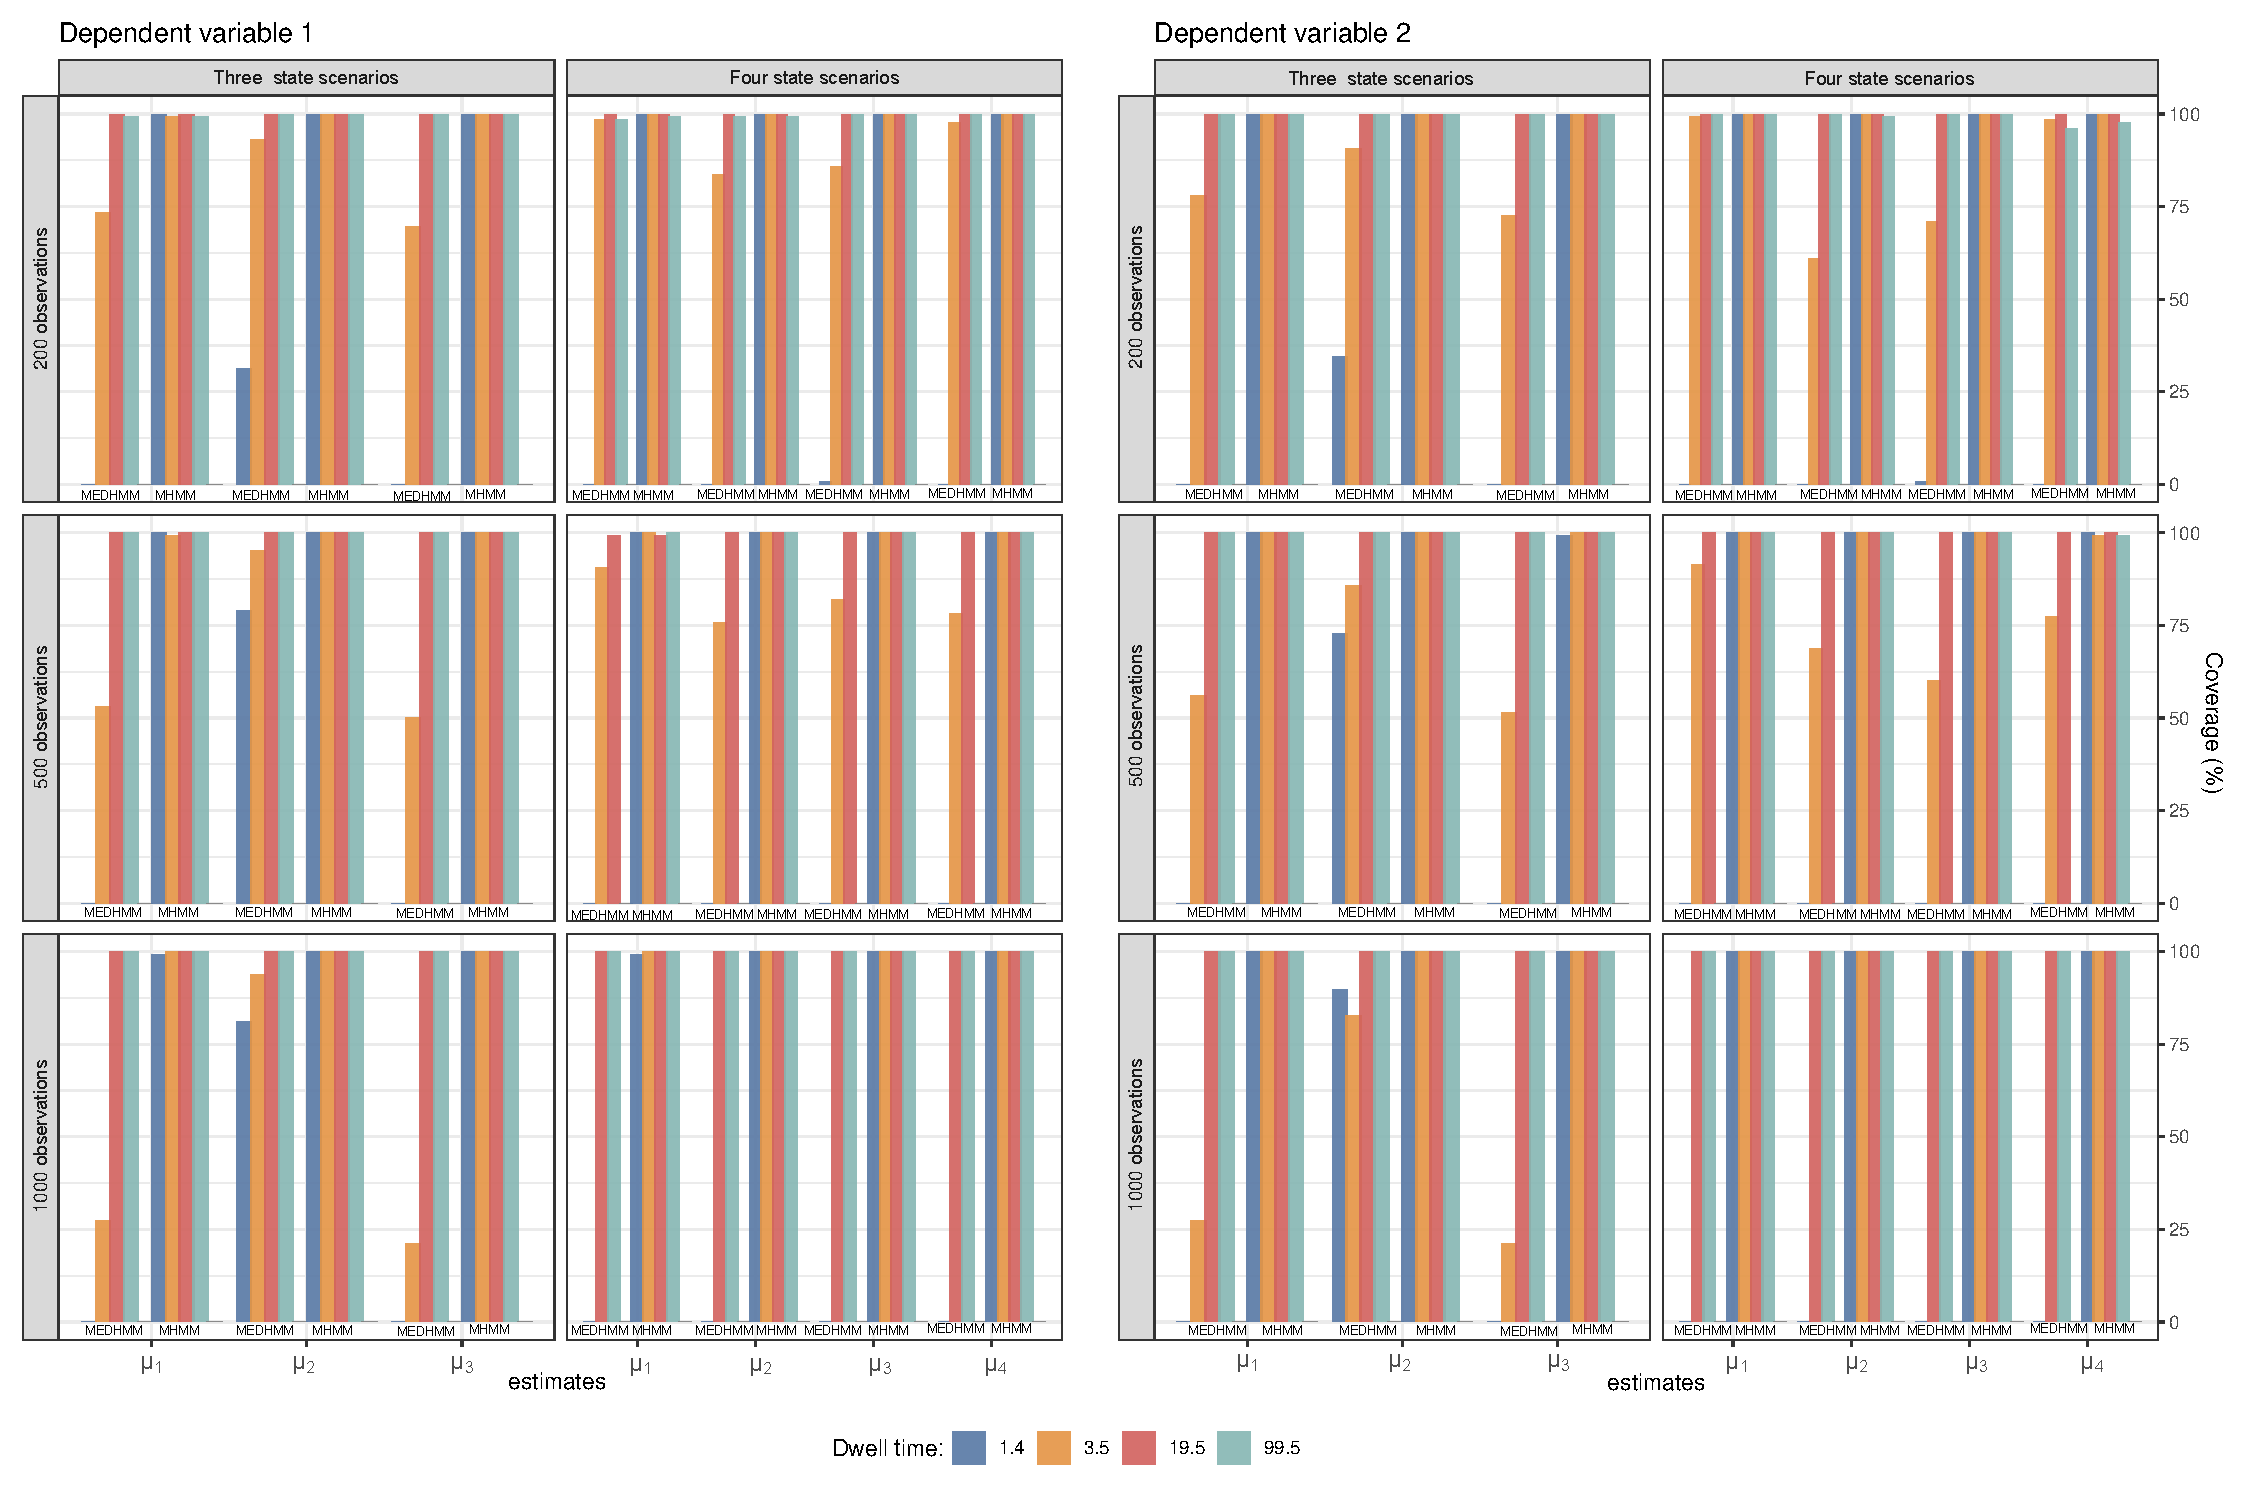
\includegraphics[width=\textwidth]{graphics/emiss_mu_cov.pdf}
     \flushleft
    \footnotesize
    \justifying
 The figure displays the Coverage over each emission distribution mean for MEDHMM and MHMM. Note that an additional scenario with varying across states dwell time was omitted here. Each panel represent a single state and observation length scenario. Colours represent the different assumed dwell time. On the x-axis the indicators of the inspected emission means are listed and within each mean parameter, the bars for MHMM and MEDHMM are shown. 
   
    \label{emiss_mu_cov}
\end{figure}



\begin{figure}[h]
\caption{The switches count for both MEDHMM \& MHMM under all simulation scenarios}
    \centering
    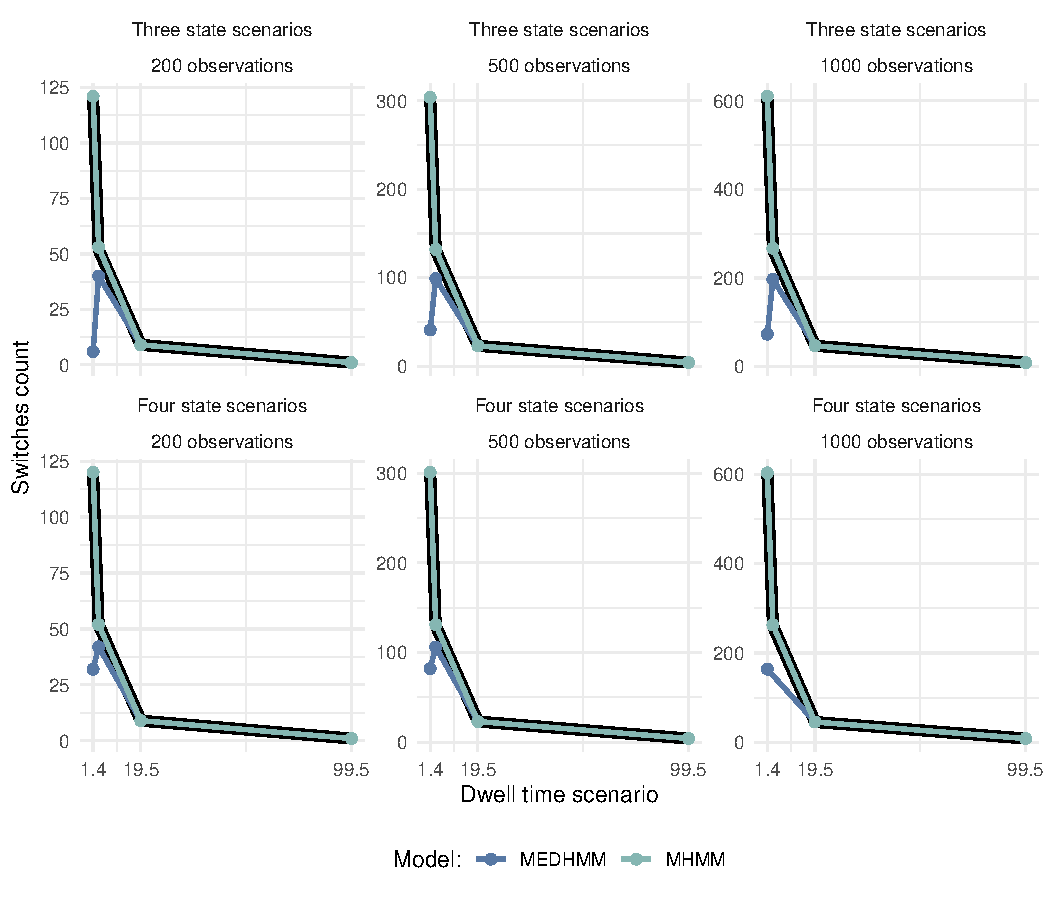
\includegraphics[width=0.9\textwidth]{graphics/switches_fin.pdf}
    \flushleft
    \footnotesize
    \justifying
    The figure displays the average count of state switches derived from local decoding (note that an additional scenario with varying across states dwell time was omitted here). Different dwell times are marked on the x-axis, and each panel represents a different observation's and state scenario. The black line indicates the in-sample true for the average number of switches.
    \label{state_switches}
\end{figure}

\begin{figure}[h]
\caption{Empirically derived dwell times}
    \centering
    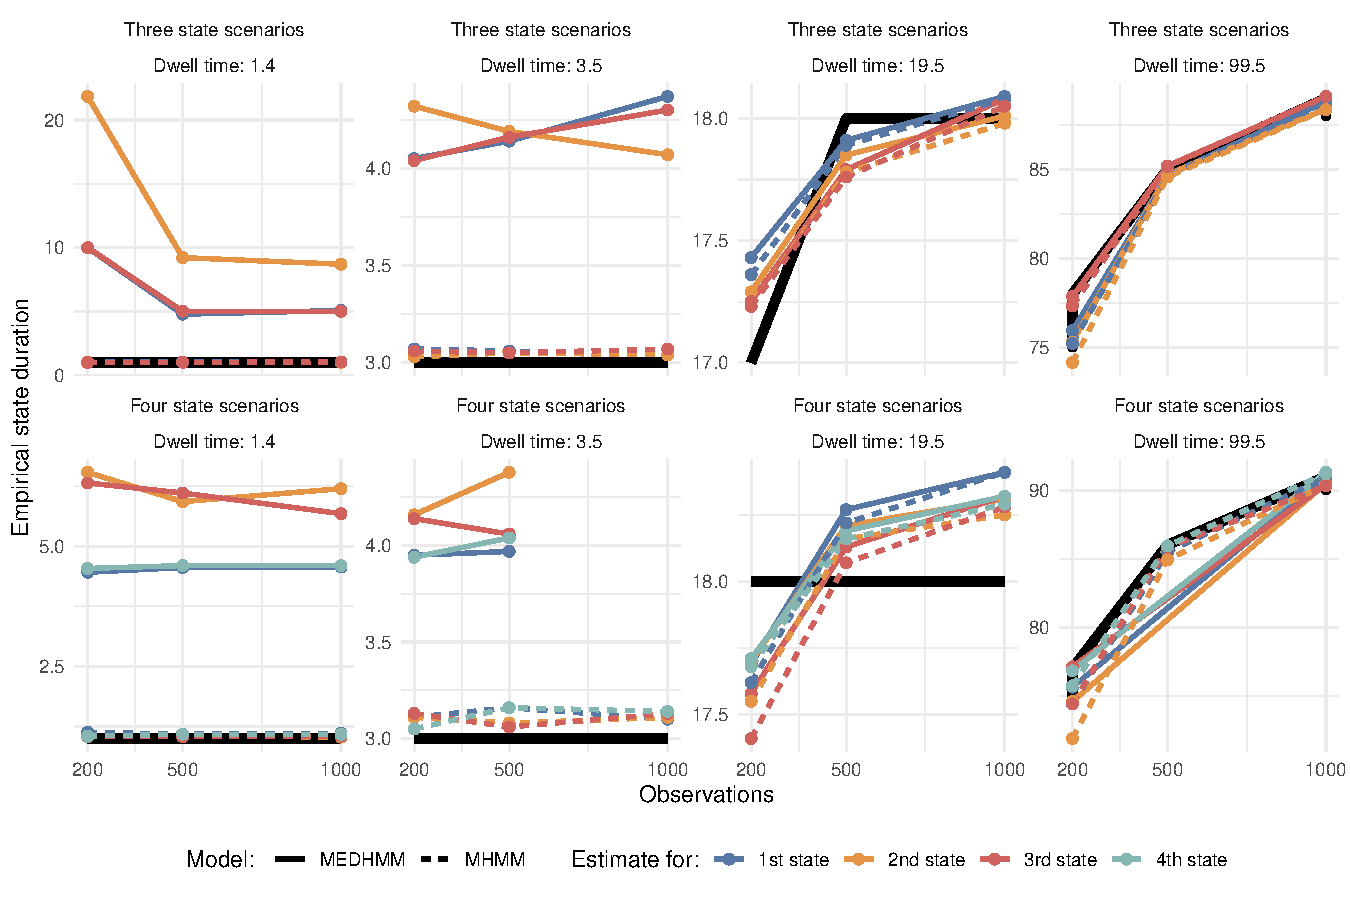
\includegraphics[width=0.8\textwidth]{graphics/dwell_time_plot.pdf}
    \flushleft
    \footnotesize
    \justifying
  The figure displays empirical state durations derived from local decoding (note that an additional scenario with varying across states dwell time was omitted here). Different lengths of observations are marked on the x-axis, and each panel represents a different dwell time and state scenario. The black line shows the average true empirical dwell time across all states, while each coloured line represents a state-specific dwell time estimate. Different models are indicated by the line type. 
    \label{empiric_dwell}
\end{figure}
